PageRank \cite{rank-page99} is an algorithm that measures the importance of nodes in a network by assigning numerical scores based on the structure of links. It finds applications in web page ranking, identifying misinformation, predicting traffic flow, and protein target identification. The increasing availability of vast amounts of data represented as graphs has led to a significant interest in parallel algorithms for computing PageRank \cite{rank-garg16, rank-nvgraph, rank-giri20, rank-sarma13}.\ignore{--- it has been implemented on multicore CPUs \cite{rank-garg16}, GPUs \cite{rank-nvgraph}, FPGAs \cite{rank-guoqiang20}, SpMV ASICs \cite{rank-sadi18}, CPU-GPU hybrids \cite{rank-giri20}, CPU-FPGA hybrids \cite{rank-li21}, and distributed systems \cite{rank-sarma13}.}

However, most real-world graph evolve with time. Here, frequent edge insertions and deletions make recomputing PageRank from scratch impractical, particularly for small, rapid changes. Existing strategies optimize by iterating from the prior snapshot's ranks, reducing the number of iterations needed for convergence. For further improvements, it is essential to recompute only the ranks of vertices likely to change. A prevalent approach involves identifying reachable vertices from the updated regions of the graph, and limiting processing to such vertices. However, if updates are randomly distributed, they often fall within dense graph regions, necessitating processing of a substantial portion of the graph.

To reduce computational effort, one can incrementally expand the set of affected vertices starting from the updated graph region, rather than processing all reachable vertices from the first iteration. Additionally, it is possible to skip processing a vertex's neighbors if the change in its rank is small and is expected to have minimal impact on the ranks of its neighboring vertices. This technical report introduces such an approach.




\subsection{Our Contributions}

This report introduces our Dynamic Frontier approach\footnote{\url{https://github.com/puzzlef/pagerank-openmp-dynamic}}, which, when given a batch update involving edge insertions and deletions, incrementally identifies affected vertices likely to undergo rank changes with minimal overhead. On a server equipped with a 64-core AMD EPYC-7742 processor, our Dynamic Frontier PageRank surpasses Static, Naive-dynamic, and Dynamic Traversal PageRank by $7.8\times$, $2.9\times$, and $3.9\times$ respectively, for uniformly random batch updates of size $10^{-7}|E|$ to $10^{-3}|E|$, where $|E|$ is the number of edges in the original graph. Additionally, our approach exhibits a performance improvement of $1.8\times$ for each doubling of threads.




%% - Use --- for a dash.
%% - Use ``camera-ready'' for quotes.
%% - Use {\itshape very} or \textit{very} for italicized text.
%% - Use \verb|acmart| or {\verb|acmart|} for mono-spaced text.
%% - Use \url{https://capitalizemytitle.com/} for URLs.
%% - Use {\bfseries Do not modify this document.} for important boldface details.
%% - Use \ref{fig:name} for referencing.

%% For a block of pre-formatted text: 
% \begin{verbatim}
%   \renewcommand{\shortauthors}{McCartney, et al.}
% \end{verbatim}

%% For a list of items:
% \begin{itemize}
% \item the ``ACM Reference Format'' text on the first page.
% \item the ``rights management'' text on the first page.
% \item the conference information in the page header(s).
% \end{itemize}

%% For a table:
% \begin{table}
%   \caption{Frequency of Special Characters}
%   \label{tab:freq}
%   \begin{tabular}{ccl}
%     \toprule
%     Non-English or Math&Frequency&Comments\\
%     \midrule
%     \O & 1 in 1,000& For Swedish names\\
%     $\pi$ & 1 in 5& Common in math\\
%     \$ & 4 in 5 & Used in business\\
%     $\Psi^2_1$ & 1 in 40,000& Unexplained usage\\
%   \bottomrule
% \end{tabular}
% \end{table}

%% For a full-width table:
% \begin{table*}
%   \caption{Some Typical Commands}
%   \label{tab:commands}
%   \begin{tabular}{ccl}
%     \toprule
%     Command &A Number & Comments\\
%     \midrule
%     \texttt{{\char'134}author} & 100& Author \\
%     \texttt{{\char'134}table}& 300 & For tables\\
%     \texttt{{\char'134}table*}& 400& For wider tables\\
%     \bottomrule
%   \end{tabular}
% \end{table*}


%% For inline math:
% \begin{math}
%   \lim_{n\rightarrow \infty}x=0
% \end{math},

%% For a numbered equation:
% \begin{equation}
%   \lim_{n\rightarrow \infty}x=0
% \end{equation}

%% For an unnumbered equation:
% \begin{displaymath}
%   \sum_{i=0}^{\infty} x + 1
% \end{displaymath}

%% For a figure:
% \begin{figure}[h]
%   \centering
%   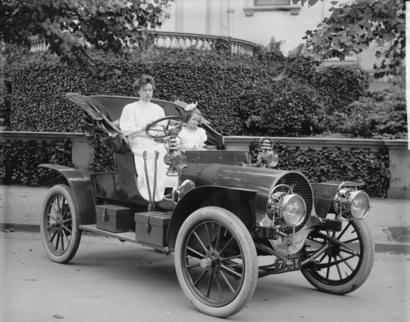
\includegraphics[width=\linewidth]{inc/sample-franklin}
%   \caption{1907 Franklin Model D roadster. Photograph by Harris \&
%     Ewing, Inc. [Public domain], via Wikimedia
%     Commons. (\url{https://goo.gl/VLCRBB}).}
%   \Description{A woman and a girl in white dresses sit in an open car.}
% \end{figure}

%% For a teaser figure.
% \begin{teaserfigure}
%   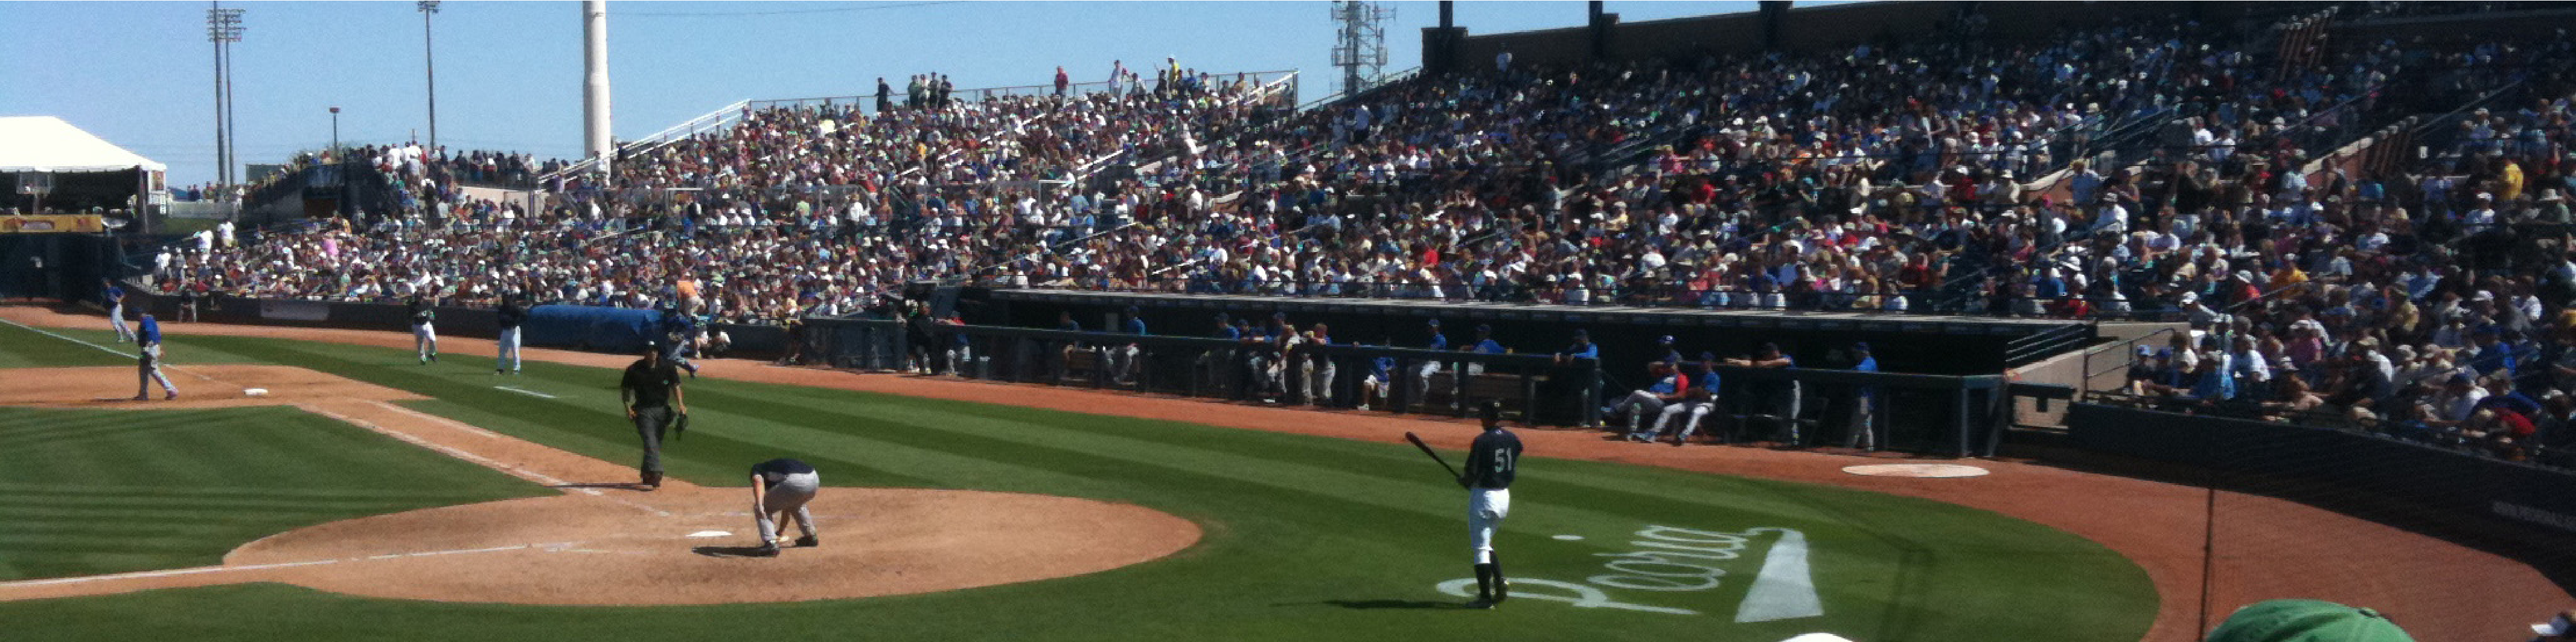
\includegraphics[width=\textwidth]{sampleteaser}
%   \caption{figure caption}
%   \Description{figure description}
% \end{teaserfigure}
